\documentclass[twoside]{uva-inf-bachelor-thesis}
\usepackage[english]{babel}

% Filling your thesis with only lorem ipsum is not advised.
\usepackage{lipsum}

\usepackage{cite}
\usepackage[style=authoryear-comp]{biblatex}
\addbibresource{Project/Thesis/LaTeX/main.bib}

% Title Page
\title{Development of an interactive experiment on the effect of sequential information on the formation of generic beliefs}
\author{Bodi Boelé}
\supervisors{Dr. Patricia Mirabile}
\signedby{-}

\begin{document}
\maketitle

\begin{abstract}
Generic statements are statements such as `ducks lay eggs', `tigers are striped', `lions have manes' and `ticks spread Lyme disease'. They express generalizations about the members of a kind. The statements lack any form of quantification and are therefore `bare'. The universally quantified version of a generic statement should be rejected by it's incorrectness; `All ducks lay eggs' which is wrong since many ducks (all male ducks) do not lay eggs. Building on earlier (ongoing) investigations on generics and alternatives, this paper will discuss the implementation of an interactive experiment including a pilot experiment.
\end{abstract}

\tableofcontents

\chapter{Introduction}
\section{Generic statements}
`Ducks lay eggs', `tigers are striped', `lions have manes' and `ticks spread Lyme disease'. These are all generic statements. Generics statements express generalizations about the members of a kind. The statements mentioned lack any form of quantification and are therefore `bare'. 

`Bare' generic statements express useful generalizations, but it is difficult to come to an unambiguous conclusion on when people think these statements are true. There is no unique critical point where people in general tend to designate a statement as true. For example when people have to judge the statement `lions have manes', the predominant conclusion will be true, although less than 50\% of lions (only the older male lions) have manes. When asked about the statement `ticks spread Lyme disease' the predominant conclusion as well would be true, even though the statement is only true for 2.7\% \parencite{rivm_2019} of tick bites that actually transfer the disease whereas 20\% of ticks carry the disease. These rather large differences in truth-conditions as investigated by \cite{leslie2011all} are caused by the generic overgeneralization effect.  

\subsection{Overgeneralization effect}
Experimental psychology has highlighted a number of biases and preferences such as the generic overgeneralization effect, the bias for people to accept a generic statement based on rare events and the biased position of people where they are more negatively biased towards non-human categories. For example people tend to classify `Men attack people' as false and `Sharks attack people' as true, even though the chance of men attacking people is vastly higher than the chance of sharks attacking people. 

The experiments conducted by \cite{leslie2011all} where they compare how people assert different formulations of generic statements, shows that people tend to falsely accept (over)generalized statements when offered a more descriptive alternative, as described in the previous section. 

\cite{tasimi2017differences} concludes that people are biased towards generics involving non-human entities. Their research also suggests that it is necessary to expand on the cognitive processes underlying these effects which is part of the goal of the overarching research project of this project.


\subsection{Impact on generic beliefs}
According to \cite{cimpian2010generic} `generic statements require little evidence for acceptance' such as the previously mentioned tick example and other striking generics like `Rottweilers maul children' and `Lions eat people' even though these statements are only true for exceptional cases. According to their research generic statements are often judged as true based on little evidence, but these implications go far beyond what is needed to accept them. This underlines the importance of the parent research on how people form these beliefs and what the effect of sequential information is on their judgement. 

\cite{van2020generics} analysed generic statements based on the intuition that other authors had formed over the years and claimed to be natural. In their paper they suggest that people tend to accept and interpret generics based on a distorted picture of it provided by the media instead of on actual frequencies.

\section{Goal}
The goal of this research project is to implement an interactive experiment on the effect of sequential information on the semantics of generic statements. The focus of this experiment will be on the importance of the learning process on the formation of beliefs regarding generic statements. This project seeks to implement an online tool which will be tested using a pilot experiment and afterwards be used in an ongoing research project by \cite{RooijSchulzGenAlt} on `Generics and Alternatives`. **(Can I refer to the `FrontiersPaperNew6' paper?) In their research \cite{RooijSchulzGenAlt} used a statistical approach to the meaning of generic sentences. In their conclusion they state that `causal impact was not tested' and that is where this thesis ties in with the investigation. This to be add ground to build a solid basis from where further theoretical work can be directed.



\chapter{Theoretical background}
Based on ... TODO



\chapter{Experimental Setup}
This experiment will build on the basis created by \cite{RooijSchulzGenAlt}. In their experiment they show the contestant a grid consisting of 2 differently coloured bugs, as shown in \ref{fig:beetle_example}
\begin{figure}
    \centering
    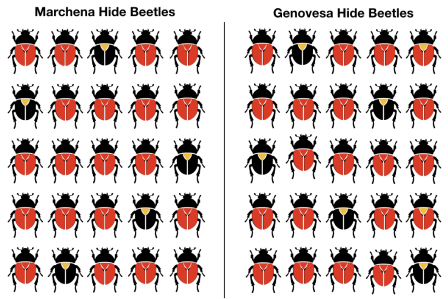
\includegraphics[width=\textwidth]{Project/Thesis/LaTeX/images/beetles_example.png}
    \caption{Sample of experiments done by \cite{RooijSchulzGenAlt}}
    \label{fig:beetle_example}
\end{figure}
\section{Data}
The data to be used will be gathered through a pilot experiment using the interactive web questionnaire created for this purpose. 


\chapter{Results}
\section{Gathering data}
\subsection{Experimental set-up}


\chapter{Discussion}
\section{Conclusions}
\section{Further research}
\section{Ethical aspects}


\printbibliography
\addcontentsline{toc}{chapter}{Bibliography}

\end{document}
